\documentclass[12pt,openright,twoside]{book}
\usepackage{graphicx}
\usepackage[a4paper,left=25mm,right=25mm,top=25mm,bottom=30mm]{geometry}
\usepackage[T1]{fontenc}
\usepackage[utf8]{inputenc}
\usepackage[romanian]{babel}
\usepackage{lmodern}
\usepackage{amsmath,amssymb,amsthm}
\usepackage{booktabs}
\usepackage{enumitem}
\usepackage{hyperref}
\usepackage{xcolor}
\usepackage{dirtree}
\usepackage{float}
\usepackage{natbib}
\usepackage{caption}
\usepackage{titlesec}
\usepackage{pdflscape}

\titleformat{\chapter}
  {\Large\bfseries}
  {}
  {0pt}
  {\LARGE}

\renewcommand{\figurename}{\textbf{Figura}}
\renewcommand{\tablename}{\textbf{Tabelul}}
\newcommand{\HRule}{\rule{\linewidth}{0.4mm}}
\renewcommand{\contentsname}{{\Huge Cuprins}}
\renewcommand{\chaptername}{{\Huge  }}

\setlength{\parindent}{0pt}
\setlength{\parskip}{0.5\baselineskip}
\setcounter{tocdepth}{2}

\begin{document}

% --- Pagina de titlu ---
\begin{titlepage}
\begin{center}


\includegraphics[width=16cm]{./antet_L.jpg}

\vspace{3cm}

\HRule \\[0.3cm]
{\Large \textsc{Simularea dinamicii moleculare a unui gaz ideal în geometrii de confinare complexe}}\\
\HRule \\[1.1cm]

\textsc{\large Lucrare de Licență}\\[4cm]

\begin{flushleft} \large
  {Absolvent} \\[0.1cm]
  Octavian \textsc{Stirbei}\\
  Facultatea de Fizică, Universitatea din București\\
  Fizică Tehnologică
\end{flushleft}

\begin{flushright} \large
  {Conducător științific} \\[0.1cm]
  Lect. dr. Dragoș \textsc{Palade}
\end{flushright}

\vfill
{\large București, 2026}

\end{center}
\end{titlepage}

% --- Pagina alba verso ---
\newpage
\vspace*{\fill}
\thispagestyle{empty}

% --- Cuprins ---
\newpage
\thispagestyle{plain}
\pagenumbering{roman}
\vspace*{\fill}
\tableofcontents

\setlength\parindent{0pt}
\setcounter{page}{0}

\newpage
\pagenumbering{arabic}

% ============================================================
\chapter{Introducere}
\label{sec:introducere}
% ============================================================

Studiul sistemelor formate din multe particule face legătura între lumea microscopică, descrisă prin mișcarea individuală a corpurilor elementare, și lumea macroscopică, în care observăm presiune, temperatură, densitate, curgere sau relaxare către echilibru. Una dintre ideile fundamentale ale fizicii statistice este că aceste mărimi macroscopice sunt efecte colective rezultate din dinamica unui număr foarte mare de grade de libertate~\cite{reif2009,halliday1975,berkeley1981}. Din acest punct de vedere, gazul ideal constituie unul dintre cele mai importante modele teoretice: suficient de simplu pentru a putea fi analizat clar și suficient de bogat pentru a ilustra mecanisme esențiale ale teoriei cinetice și ale echilibrului statistic~\cite{maxwell1860}.

Din punct de vedere microscopic, particulele unui gaz ideal nu exercită forțe unele asupra altora; mișcarea lor este liberă între două evenimente succesive de contact cu frontiera. Dacă nu există interacții interparticulare, singurele elemente care pot organiza dinamica sunt condițiile inițiale și condițiile la limită. În modelul studiat aici, condițiile la limită nu înseamnă doar forma spațiului accesibil, ci și natura fizică a frontierelor: un perete poate reflecta elastic, poate atenua selectiv componentele vitezei sau poate acționa ca o frontieră termalizantă care menține particulele în contact termic cu mediul~\cite{cercignani1988}.

Această observație are o consecință importantă: în analiza unui gaz ideal confinat, pereții nu reprezintă doar un detaliu geometric, ci o componentă constitutivă a modelului fizic. Aceeași geometrie poate conduce la răspunsuri diferite dacă suprafețele care o delimitează au proprietăți de ricoșeu, disipare sau termalizare diferite. Prin urmare, orice neomogenitate spațială sau timp de relaxare caracteristic poate fi corelat direct cu forma domeniului și cu modul de interacție la frontieră~\cite{cercignani1988,kogan1969}.

Interesul pentru asemenea probleme nu este doar teoretic. Multe sisteme reale implică particule sau molecule care se deplasează în medii confinate: micro-canale, materiale poroase, sisteme coloidale, medii biologice aglomerate, structuri nanometrice sau volume compartimentate~\cite{squires2005,drescher2011}. În geometrii complexe, chiar și fără interacții interparticulare, geometria poate induce o dinamică bogată: unele regiuni sunt explorate rapid, altele mai greu; canale înguste pot crea bariere entropice care controlează transportul fără niciun potențial extern. Astfel, forma spațiului devine ea însăși un mecanism activ de selecție și reorganizare a traiectoriilor.

O întrebare centrală în fizica transportului confinat este dacă o geometrie asimetrică, combinată cu proprietăți materiale diferite ale pereților, poate produce un curent net staționar (o stare de neechilibru staționar, NESS) fără niciun dezechilibru extern. Această idee a fost formulată clasic de Feynman prin modelul clichetului termic~\cite{feynman1963}: un mecanism asimetric ar putea, în principiu, rectifica fluctuațiile termice și produce lucru mecanic net. Analiza termodinamică arată însă că la temperatură uniformă acest lucru este imposibil: clichetul nu poate funcționa ca motor fără o sursă externă de dezechilibru, altfel al doilea principiu ar fi violat~\cite{feynman1963,parrondo1996,magnasco1993,reimann2002}.

Motoarele Browniene reale, fie moleculare biologice, fie artificiale, produc flux net numai prin alimentare chimică sau prin gradient termic, nu prin geometrie singură~\cite{astumian2002,hanggi2009}. Un exemplu fizic direct este pompa Knudsen~\cite{knudsen1909,karniadakis2005}: un dispozitiv fără piese mobile care pompează gaz printr-un gradient termic în regim rarefiat ($\text{Kn} = \lambda/L \gtrsim 0{,}1$, unde $\lambda$ este drumul liber mediu și $L$ dimensiunea caracteristică a canalului), unde coliziunile individuale particulă--perete domină transportul față de coliziunile interparticulare. Simulările din această lucrare operează în regimul opus: densitatea particulelor este suficient de mică pentru a neglija coliziunile binare, dar $\text{Kn}$ nu este în regim Knudsen pur — mecanismul de transport este dominat de dinamica Langevin în volum, nu de efecte de gaz rarefiat la scară $\lambda$. Și în cazul pompei Knudsen, sursa NESS este gradientul termic extern, nu geometria.

În modelul adoptat, mișcarea în volum este descrisă prin ecuația Langevin~\cite{langevin1908,einstein1905}: pe lângă zborul liber, fiecare particulă este supusă unui termen de fricțiune și unui zgomot termic calibrat prin teorema fluctuație--disipație~\cite{kubo1966}. Parametrul $\gamma$ controlează regimul dinamic: la $\gamma$ mic sistemul este cvasi-balistic (drumul liber mediu lung), la $\gamma$ mare particulele sunt puternic cuplate la rezervorul termic și se comportă difuziv~\cite{gardiner2009}. Timpul caracteristic de relaxare a vitezei este $\tau_v = m/\gamma$; în unitățile reduse ale simulării ($m = k_BT = 1$), valoarea $\gamma = 1$ produce $\tau_v = 1$, iar la pasul de integrare $\Delta t = 0{,}001$ vitezele sunt decorelate după aproximativ $10^3$ pași. La $\gamma = 0{,}01$, $\tau_v = 100$ și particulele parcurg distanțe lungi balistic înainte să termalizeze, cerând rulări mult mai lungi pentru a acumula statistică relevantă.

O distribuție Maxwell--Boltzmann a vitezelor este o condiție necesară, dar nu suficientă pentru echilibrul termodinamic. Testul mai sensibil este bilanțul detaliat: la echilibru, rata de tranziție între oricare două stări trebuie să fie egală cu rata inversă~\cite{onsager1931,maes2021}. Operațional, geometria este împărțită în regiuni distincte (\texttt{CUBE\_L}, \texttt{FUN\_1}\,--\,\texttt{FUN\_6}, \texttt{CUBE\_R}, \texttt{RET}), iar fiecare traversare a unui tracer dintr-o regiune în alta este înregistrată. Din frecvențele de tranziție se construiește matricea $C_{ij}$ și se calculează curentul net pe ciclul principal: $J_\text{loop} = C_{LF} C_{FR} C_{Rr} - C_{rR} C_{RF} C_{FL}$, unde indicii urmăresc sensul CUBE\_L $\to$ FUNNELS $\to$ CUBE\_R $\to$ RET $\to$ CUBE\_L. Un curent net $J_\text{loop} \neq 0$ indică ruperea bilanțului detaliat și prezența unui NESS real; la echilibru termodinamic, $J_\text{loop} = 0$ cu precizie statistică~\cite{jiang2004,maes2021}.

Geometriile complexe nu sunt tractabile analitic complet; urmărirea statisticilor de transport necesită simularea explicită a unui ansamblu de $N$ particule pe intervale lungi de timp. Pachetul \texttt{brownian\_sim} dezvoltat în această lucrare permite rularea sistematică a diferitelor combinații de geometrie, model de perete și regim dinamic, cu rezultate reproductibile și verificate prin teste unitare~\cite{allen2017,frenkel2002}. Înainte de orice simulare în geometria complexă, fiecare componentă a codului este validată independent: modelele de perete sunt testate față de distribuția teoretică Maxwell--Boltzmann, algoritmul de integrare este verificat prin conservarea valorii $\langle v^2 \rangle = 3k_BT/m$, iar detectarea coliziunilor este testată pe geometrii simple cu soluție analitică. Această strategie de validare în trepte asigură că rezultatele din geometria complexă reflectă fizica modelului, nu artefacte numerice.

Lucrarea de față testează această limită: un gaz ideal cu dinamică Langevin într-o geometrie asimetrică formată din două camere cubice (\texttt{CUBE\_L} și \texttt{CUBE\_R}), conectate prin două căi distincte: un canal cu pâlnie compus din șase secțiuni cilindrice cu secțiune variabilă (\texttt{FUN\_1}\,--\,\texttt{FUN\_6}), orientat de-a lungul axei $y$, și un canal de retur cilindric (\texttt{RET}), orientat de-a lungul axei $x$. Pereții sunt termalizanți la aceeași temperatură $T$, dar coeficienții materiali $(e_n, \beta_t)$ pot diferi între piese, introducând o asimetrie în modul în care particulele interacționează cu frontierele celor două căi. Această geometrie a fost aleasă tocmai pentru că oferă un ciclu închis bine definit, cu o asimetrie controlabilă între calea directă (pâlnie) și calea de retur, permițând testarea riguroasă a bilanțului detaliat prin calculul $J_\text{loop}$. Întrebarea centrală este dacă geometria asimetrică și eterogenitatea materială a frontierelor pot produce un curent net $J_\text{loop} \neq 0$ prin ciclu, sau dacă bilanțul detaliat impune $J_\text{loop} = 0$ indiferent de configurație.

Structura tezei urmează această logică. Capitolul~\ref{sec:fundamente} răspunde la întrebarea \textit{ce model fizic folosim}: prezintă modelul gazului ideal, dinamica Langevin și procesul Ornstein--Uhlenbeck, modelele de interacție particulă--perete (elastic, OUBounce, Maxwell diffuse) și observabilele statistice prin care regimul staționar este caracterizat. Capitolul~\ref{sec:model} răspunde la întrebarea \textit{cum este implementat}: arhitectura pachetului \texttt{brownian\_sim}, reprezentarea geometriei prin primitive SDF, algoritmul de integrare BAOAB și suita de teste de verificare care validează fiecare componentă în parte. Capitolul~\ref{sec:rezultate} răspunde la întrebarea \textit{ce observăm}: rezultatele simulărilor de la cazul de referință (cutie simplă) la geometria complexă, cu analiza distribuției vitezelor, a ocupanței camerelor, a curentului $J_\text{loop}$ și a matricei de tranziții pentru fiecare configurație. Capitolul~\ref{sec:concluzii} sintetizează răspunsul la întrebarea centrală și indică direcțiile de extindere către sisteme cu adevărat în neechilibru.

% ============================================================
\chapter{Fundamente teoretice}
\label{sec:fundamente}
% ============================================================

\section{Modelul gazului ideal}

Modelul de gaz ideal constituie una dintre idealizările fundamentale ale fizicii statistice și ale teoriei cinetice~\cite{reif2009,cercignani1988,plavitu_termice,stefan_termice,ciobanu_statistica}. Importanța sa nu provine din faptul că ar descrie exhaustiv un gaz real, ci din faptul că izolează un set minim de ingrediente fizice prin care relația dintre dinamică microscopică și comportament macroscopic poate fi analizată clar. În cadrul acestei lucrări, modelul este folosit ca punct de plecare pentru studiul influenței combinate a geometriei de confinare și a proprietăților materiale ale frontierelor asupra evoluției unui ansamblu de particule.

Considerăm un sistem alcătuit dintr-un număr mare de particule identice, fiecare având masă constantă $m$. Starea microscopică a sistemului este determinată, la un moment dat, de pozițiile $\mathbf{r}_i$ și vitezele $\mathbf{v}_i$ ale particulelor, cu $i=1,\dots,N$. Modelul se sprijină pe următoarele ipoteze pentru mișcarea în volum:

\begin{enumerate}[label=\arabic*.]
    \item particulele au masă constantă și sunt tratate drept punctiforme sau cu volum propriu neglijabil;
    \item între particule nu acționează forțe directe și nu au loc coliziuni binare;
    \item între două interacții succesive cu frontiera, fiecare particulă se deplasează liber;
    \item domeniul accesibil este finit și este delimitat de pereți rigizi;
    \item în forma ideală elementară a modelului, ciocnirile particulă--perete sunt perfect elastice.
\end{enumerate}

Aceste ipoteze simplifică puternic problema și permit separarea efectelor pur geometrice de efectele datorate interacțiunilor interparticulare. Câștigul principal este claritatea interpretării: dacă particulele nu se ciocnesc între ele, atunci rolul dominant este jucat de forma domeniului și de condițiile la limită.

Se pierde însă realismul complet al unui gaz real. În absența coliziunilor interparticulare, modelul nu descrie în mod direct termalizarea internă, transportul vâscos în sens strict sau apariția unei distribuții Maxwell--Boltzmann prin schimburi reciproce de impuls. Din acest motiv, echilibrul trebuie înțeles ca un regim staționar al observabilelor relevante pentru dinamica și confinarea considerate.

În formularea extinsă considerată aici, modelul de bază este completat prin termeni stocastici și prin condiții la limită mai generale decât ricoșeul perfect elastic. În forma deterministă cea mai simplă, fiecare particulă se deplasează rectiliniu și uniform între două interacții succesive cu frontiera:

\begin{equation}
    m\frac{d^2\mathbf{r}}{dt^2}=\mathbf{0}.
\end{equation}

Echivalent, viteza este constantă pe fiecare interval de zbor liber,

\begin{equation}
    \frac{d\mathbf{v}}{dt}=\mathbf{0},
\end{equation}

astfel încât poziția este dată de relația

\begin{equation}
    \mathbf{r}(t)=\mathbf{r}_0+\mathbf{v}t.
\end{equation}

Aceasta arată că, în interiorul domeniului, traiectoria particulei nu este complicată prin mecanisme interne: întregul caracter nebanal al dinamicii provine din succesiunea interacțiilor cu pereții sau, în extensia stocastică, din acțiunea termenilor de fricțiune și zgomot.

În modelul clasic ideal, pereții sunt considerați rigizi și perfect elastici. Fie $\hat{\mathbf{n}}$ normala unitară la suprafață, orientată spre interiorul domeniului. Viteza incidentă $\mathbf{v}$ se poate descompune într-o componentă normală și una tangențială,

\begin{equation}
    \mathbf{v}=\mathbf{v}_n+\mathbf{v}_t, \qquad
    \mathbf{v}_n=(\mathbf{v}\cdot\hat{\mathbf{n}})\hat{\mathbf{n}},
    \qquad
    \mathbf{v}_t=\mathbf{v}-\mathbf{v}_n.
\end{equation}

Pentru o reflexie speculară ideală, componenta normală își schimbă semnul, iar componenta tangențială se conservă:

\begin{equation}
    \mathbf{v}'=\mathbf{v}-2(\mathbf{v}\cdot\hat{\mathbf{n}})\hat{\mathbf{n}}.
    \label{eq:specular_reflection}
\end{equation}

Aceasta implică conservarea energiei cinetice~\cite{cercignani1988,kogan1969}, $|\mathbf{v}'|^2=|\mathbf{v}|^2$: peretele nu disipă energie, ci doar redirecționează mișcarea.

\section{Dinamica Langevin și procesul Ornstein--Uhlenbeck}

Modelul fizic adoptat aici nu se limitează la mișcarea rectilinie uniformă între ricoșeuri. El introduce în volum o dinamică de tip Langevin pentru viteză~\cite{langevin1908,einstein1905,lemons1997}, ceea ce înseamnă că particulele sunt supuse simultan unui termen disipativ și unui termen de zgomot termic. La nivel continuu, modelul standard este

\begin{equation}
    \frac{d\mathbf{r}}{dt}=\mathbf{v},
\end{equation}

\begin{equation}
    m\frac{d\mathbf{v}}{dt}=-\gamma\mathbf{v}+\sqrt{2\gamma k_B T}\,\boldsymbol{\eta}(t),
    \label{eq:langevin_velocity}
\end{equation}

unde $\gamma$ este coeficientul de fricțiune, $T$ temperatura efectivă a rezervorului termic, iar $\boldsymbol{\eta}(t)$ este un zgomot gaussian alb cu medie nulă și corelații

\begin{equation}
    \langle \eta_\alpha(t) \rangle = 0,
    \qquad
    \langle \eta_\alpha(t)\eta_\beta(t') \rangle = \delta_{\alpha\beta}\,\delta(t-t').
\end{equation}

Termenul proporțional cu $-\gamma\mathbf{v}$ reprezintă efectul disipativ al unui mediu efectiv. Termenul aleator descrie fluctuațiile microscopice ale aceluiași mediu și introduce agitație termică. Prin urmare, modelul nu reprezintă un gaz complet izolat, ci un ansamblu de particule în contact cu un rezervor termic efectiv.

Ecuația Langevin liniară pentru viteză definește un proces de tip Ornstein--Uhlenbeck~\cite{uhlenbeck1930}. Din punct de vedere matematic, acesta este un proces gaussian, markovian, care relaxează către o distribuție staționară~\cite{vankampen2007,risken1989}. Scara caracteristică de timp este

\begin{equation}
    \tau_v = \frac{m}{\gamma}.
\end{equation}

Dacă timpul de observație este mult mai mic decât $\tau_v$, mișcarea păstrează un caracter mai apropiat de regimul balistic. Dacă este mult mai mare, vitezele sunt puternic influențate de rezervorul termic și de zgomot.

Distribuția staționară a vitezelor în modelul Langevin este gaussiană și compatibilă cu distribuția Maxwelliană pe componente. Amplitudinea zgomotului $\sqrt{2\gamma k_B T}$ nu este arbitrară; ea exprimă teorema fluctuație--disipație~\cite{kubo1966,marconi2008}: aceeași interacție efectivă cu mediul care introduce fricțiune trebuie să introducă și fluctuații termice cu amplitudine corelată precis, astfel încât regimul staționar să fie compatibil cu temperatura $T$~\cite{gardiner2009}.

\section{Modele de interacție particulă--perete}

Un alt element teoretic important este faptul că interacția cu peretele nu este tratată mereu ca reflexie perfect elastică. În locul legii ideale, se folosește un model generalizat în care componentele normală și tangențială ale vitezei după ricoșeu sunt modificate diferit. Dacă descompunem viteza incidentă sub forma $\mathbf{v}=\mathbf{v}_n+\mathbf{v}_t$, modelul generalizat este

\begin{equation}
    \mathbf{v}' = -e_n\mathbf{v}_n + \beta_t \mathbf{v}_t,
    \label{eq:general_wall_bounce}
\end{equation}

unde $e_n \in [0,1]$ este coeficientul de restituție normal, iar $\beta_t \in [0,1]$ este un factor de amortizare tangențială. Cazul ideal perfect elastic apare ca situație particulară pentru $e_n=\beta_t=1$~\cite{cercignani1971,kogan1969}.

Un rezultat imediat al formulei~\eqref{eq:general_wall_bounce} este bilanțul energetic la ricoșeu:

\begin{equation}
    |\mathbf{v}'|^2 = e_n^2 |\mathbf{v}_n|^2 + \beta_t^2 |\mathbf{v}_t|^2.
\end{equation}

Energia cinetică se conservă numai dacă ambele coeficiente sunt egale cu unu. În toate celelalte cazuri, coliziunea cu peretele devine disipativă: peretele nu mai este doar un reflector geometric, ci poate acționa ca element de frânare și de selecție a dinamicii.

Codul conține și o extensie termalizantă a interacției cu peretele, notată OUBounce. Din punct de vedere fizic, aceasta poate fi interpretată ca o condiție la limită termalizantă: particula nu doar ricoșează, ci primește la contact și o contribuție stochastică compatibilă cu temperatura locală a peretelui. Componenta tangențială urmează

\begin{equation}
    \mathbf{v}_t' = \beta_t\mathbf{v}_t + \sqrt{1-\beta_t^2}\,s\,\boldsymbol{\xi}_t,
\end{equation}

iar componenta normală

\begin{equation}
    v_n' = e_n |v_n^{\text{in}}| + \sqrt{1-e_n^2}\,s\,\xi_n,
    \qquad v_n' > 0,
\end{equation}

unde $s=\sqrt{k_B T / m}$ și $\boldsymbol{\xi}_t$, $\xi_n$ sunt variabile gaussiene. Factorul $\sqrt{1-e_n^2}$ la zgomotul normal și $\sqrt{1-\beta_t^2}$ la cel tangential sunt impuși de relația fluctuație--disipație: pentru ca distribuția staționară a vitezelor după ricoșeu să fie Maxwell--Boltzmann la temperatura $T$, amplitudinea zgomotului trebuie calibrată precis față de disipare.

Un caz limită important al modelului termalizant este condiția la limită Maxwell diffuse~\cite{maxwell1879,cercignani1988}. Spre deosebire de OUBounce, unde viteza de ieșire depinde prin termenul $e_n|v_n^\text{in}|$ de viteza incidentă, condiția Maxwell diffuse presupune că particula care lovește peretele uită complet viteza de intrare. Viteza de ieșire este trasă independent din distribuția termică a peretelui:

\begin{equation}
    \mathbf{v}_t' \sim \mathcal{N}(0,\, k_BT/m)\text{ în planul tangent},
    \label{eq:maxwell_diffuse_t}
\end{equation}

\begin{equation}
    v_n' \sim \text{Rayleigh}(\sigma),\quad \sigma = \sqrt{k_BT/m},\quad v_n' > 0.
    \label{eq:maxwell_diffuse_n}
\end{equation}

Distribuția Rayleigh pentru componenta normală (nu semi-gaussiană) apare din ponderea cu fluxul de particule: o particulă cu viteză normală $v_n'$ mai mare traversează suprafața mai des, deci probabilitatea de emisie este proporțională cu $v_n' \exp(-v_n'^2/2\sigma^2)$, ceea ce dă exact distribuția Rayleigh~\cite{cercignani1988,kogan1969}. Această proprietate garantează bilanțul detaliat la nivel de coliziune individuală: rata de tranziție $\mathbf{v} \to \mathbf{v}'$ este egală cu rata inversă $\mathbf{v}' \to \mathbf{v}$, o condiție mai puternică decât simpla termalizare marginală~\cite{cercignani1971,maes2021}. Consecința directă este că un sistem cu pereți Maxwell diffuse la aceeași temperatură $T$ satisface $J_\text{loop} = 0$ indiferent de geometrie sau de distribuția materialelor pe frontieră.

\section{Echilibru statistic, distribuții staționare și presiune}

În modelul analizat aici, noțiunea de echilibru statistic trebuie discutată separat pentru două niveluri. În modelul balistic cu ricoșeu elastic ideal, echilibrul înseamnă în primul rând stabilizarea distribuțiilor spațiale și absența variațiilor sistematice ale observabilelor macroscopice relevante. În modelul extins cu dinamică Langevin și perete termalizant, noțiunea de staționaritate devine mai apropiată de sensul clasic al echilibrului pentru o dinamică în contact cu un rezervor termic.

În absența coliziunilor interparticulare, distribuția Maxwell--Boltzmann nu apare ca rezultat inevitabil al modelului pur balistic. Ea apare natural doar atunci când există un mecanism efectiv de redistribuire statistică a vitezelor, fie prin coliziuni între particule, fie prin cuplarea la un rezervor termic. În modelul extins considerat aici, tocmai termenii Langevin și ricoșeul stocastic la perete joacă acest rol.

Din punct de vedere spațial, echilibrul sau regimul staționar se exprimă prin faptul că distribuția de poziții nu mai prezintă o derivă sistematică în timp. Totuși, în geometrii complexe, chiar și în regim staționar pot apărea densități locale diferite și timpi de rezidență diferiți. Prin urmare, staționaritatea nu trebuie confundată automat cu uniformitatea absolută.

Presiunea este una dintre cele mai importante punți între descrierea microscopică și cea macroscopică. În teoria cinetică, ea este interpretată ca rezultatul transferului de impuls către pereți produs de coliziunile particulelor cu frontiera~\cite{cercignani1988}. Pentru o suprafață de arie $A$, dacă pe un interval de timp $\Delta t$ au loc coliziuni care produc variații de impuls normal $\Delta p_{n,k}$, atunci presiunea medie poate fi exprimată conceptual prin relația

\begin{equation}
    P \sim \frac{1}{A\,\Delta t}\sum_k \Delta p_{n,k}.
\end{equation}

Această formulă exprimă ideea fizică centrală: presiunea este flux de impuls prin frontieră.

\section{Observabile statistice din dinamica moleculară}
\label{subsec:observabile}

Odată ce modelul fizic și regulile de interacție cu frontiera sunt stabilite, devine esențial să se precizeze ce se măsoară efectiv din simulare. Observabilele statistice sunt mărimi extrase din ansamblul de traiectorii ale particulelor și reprezintă interfața dintre descrierea microscopică și concluzia fizică.

\paragraph{Distribuția vitezelor și repartiția Maxwell--Boltzmann.}
Cea mai directă verificare a regimului staționar este distribuția modulului vitezei. Pentru un sistem în echilibru termic la temperatura $T$, distribuția Maxwell--Boltzmann prevede

\begin{equation}
    f(v) = 4\pi \left(\frac{m}{2\pi k_B T}\right)^{3/2} v^2 \exp\!\left(-\frac{mv^2}{2k_B T}\right),
    \label{eq:maxwell_boltzmann}
\end{equation}

valabilă în trei dimensiuni~\cite{reif2009,pathria2011,mandl2008}. O condiție echivalentă și mai ușor de verificat numeric este că fiecare componentă cartesiană a vitezei urmează o distribuție gaussiană cu medie nulă și varianță $k_B T / m$, sau în termeni de valoare medie pătratică,

\begin{equation}
    \langle v^2 \rangle = \frac{3k_B T}{m}.
    \label{eq:equipartitie}
\end{equation}

Această relație servește drept criteriu principal de validare. În simulările cu $N=30\,000$ de particule efectuate în această lucrare, valoarea măsurată la echilibru este $\langle v^2 \rangle = 3{,}016$, în acord cu valoarea teoretică 3{,}000 pentru $m=k_B T=1$.

\paragraph{Densitatea spațială.}
Distribuția spațială a particulelor este descrisă de densitatea locală $\rho(\mathbf{r},t)$, definită operațional ca numărul de particule per unitate de volum într-o vecinătate a punctului $\mathbf{r}$ la momentul $t$. Distribuția uniformă în spațiu este o proprietate a regimului staționar în absența unor forțe externe sau a unor frontiere disipative asimetrice.

\paragraph{Temperatura locală.}
O extensie a observabilei de mai sus constă în calculul temperaturii locale pe subregiuni ale domeniului:

\begin{equation}
    T_{\text{loc}}(\mathbf{r}) = \frac{m}{3k_B}\langle v^2 \rangle_{\mathbf{r}},
\end{equation}

unde media este efectuată doar asupra particulelor aflate în vecinătatea punctului $\mathbf{r}$. Dacă toate frontierele sunt termalizante, temperatura locală trebuie să fie uniformă și egală cu temperatura de referință $T$.

\paragraph{Deplasarea medie pătratică.}
Deplasarea medie pătratică (MSD) este definită ca

\begin{equation}
    \text{MSD}(t) = \left\langle \left|\mathbf{r}(t) - \mathbf{r}(0)\right|^2 \right\rangle,
    \label{eq:msd}
\end{equation}

unde media este efectuată pe ansamblul de particule. Un regim balistic produce $\text{MSD}(t)\sim t^2$, iar un regim difuziv produce $\text{MSD}(t)\sim t$ la timpi lungi~\cite{einstein1905,smoluchowski1906,kubo1991,michalet2010}.

\paragraph{Fluxul de coliziuni și presiunea.}
Numărul de coliziuni cu fiecare porțiune a frontierei, combinat cu variația de impuls la fiecare impact, permite reconstituirea fluxului de impuls și a presiunii locale. Aceste statistici sunt utile în special pentru compararea comportamentului diferitelor secțiuni materiale ale geometriei și pentru identificarea asimetriilor induse de ricoșeu disipativ sau termalizant.

Împreună, aceste observabile oferă o descriere completă a regimului staționar și a dinamicii de relaxare, permițând trasarea unui răspuns clar la întrebările fizice centrale.

% ============================================================
\chapter{Model numeric și implementare}
\label{sec:model}
% ============================================================

\section{Arhitectura pachetului de simulare}

Simulările din această lucrare sunt realizate cu pachetul Python \texttt{brownian\_sim}, organizat după principiul separării responsabilităților~\cite{alder1959,allen2017,frenkel2002}: fiecare subpachet are un singur rol bine delimitat, iar dependențele sunt unidirecționale. Structura pe disc este prezentată în Figura~\ref{fig:dirtree}.

\begin{figure}[H]
\dirtree{%
.1 brownian\_sim/.
.2 geometry/.
.3 primitives.py \DTcomment{Box, CylX, CylY — SDF + snap\_and\_normal}.
.3 assembly.py \DTcomment{uniune de primitive, sampling uniform}.
.3 presets/ \DTcomment{simple\_box, loop\_chambers}.
.2 physics/.
.3 wall\_models.py \DTcomment{Elastic, Damped, OU, MaxwellDiffuse}.
.3 dynamics.py \DTcomment{LangevinIntegrator — pas BAOAB}.
.3 backend.py \DTcomment{selector NumPy / CuPy}.
.2 materials/.
.3 wall\_material.py \DTcomment{WallMaterial(e\_n, beta\_t)}.
.2 simulation/.
.3 engine.py \DTcomment{bucla principală time-stepping}.
.3 substepping.py \DTcomment{CFL adaptiv, detecție coliziuni}.
.3 sampler.py \DTcomment{inițializare poziții și viteze}.
.2 io/.
.3 gsd\_writer.py \DTcomment{trajectorie HOOMD-GSD}.
.3 csv\_logger.py \DTcomment{piece\_counts + transitions}.
.2 analysis/.
.3 equilibrium.py \DTcomment{$\langle v^2\rangle$, distribuție MB}.
.3 msd.py \DTcomment{deplasare medie pătratică}.
.3 transitions.py \DTcomment{matrice tranziții brute}.
.3 ness.py \DTcomment{bilanț detaliat, $J_\text{loop}$, verdict echilibru/NESS}.
.3 wall\_stats.py \DTcomment{frecvență coliziuni per regiune}.
.2 scripts/.
.3 run\_sim.py \DTcomment{CLI: python -m brownian\_sim.scripts.run\_sim}.
.3 preview\_geometry.py \DTcomment{export PNG geometrie}.
}
\caption{Structura pachetului \texttt{brownian\_sim}. Fiecare subpachet are responsabilitate unică; dependențele curg de sus în jos.}
\label{fig:dirtree}
\end{figure}

Fluxul complet de la configurație la rezultate este ilustrat în Figura~\ref{fig:arhitectura}. Utilizatorul specifică parametrii simulării într-un fișier YAML; \texttt{run\_sim.py} construiește obiectele corespunzătoare și le injectează în motorul de simulare; rezultatele sunt scrise simultan în format GSD (pentru trajectorii) și CSV (pentru statistici de ocupare și tranziții între regiuni); modulele de analiză procesează independent aceste ieșiri.

\begin{figure}[H]
\centering
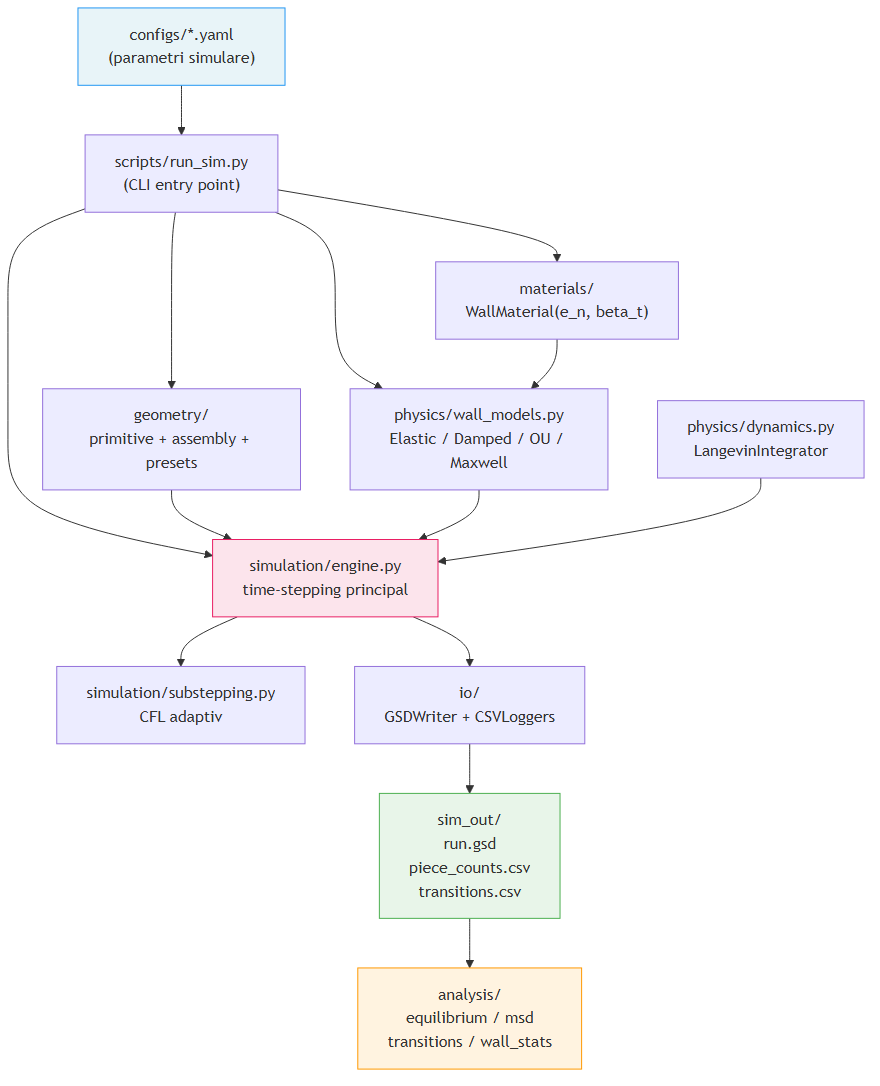
\includegraphics[width=0.90\textwidth]{diagrama_arhitectura.png}
\caption{Diagrama fluxului de date în \texttt{brownian\_sim}. Albastru: intrare (YAML); roz: motor de simulare; verde: ieșiri; portocaliu: analiză post-procesare.}
\label{fig:arhitectura}
\end{figure}

O simulare se lansează cu o singură comandă:

\begin{verbatim}
python -m brownian_sim.scripts.run_sim \
    --config configs/loop_ou_hetero_long.yaml
\end{verbatim}

Toate configurațiile din această lucrare sunt fișiere YAML versionabile, reproducibile prin specificarea seminței (\texttt{seed: 42}). Separarea dintre configurație și cod permite rularea sistematică a mai multor experimente fără modificarea surselor.

Simularea urmărește pozițiile și vitezele unui număr $N$ de particule într-un domeniu tridimensional. Parametrii principali sunt rezumați în Tabelul~\ref{tab:params}.

\begin{table}[ht]
\centering
\begin{tabular}{lll}
\toprule
Parametru & Valoare & Semnificație \\
\midrule
$N$ & 30\,000 & număr de particule \\
$\Delta t$ & 0.001 & pas temporal de bază \\
$k_B T$ & 1.0 & temperatură efectivă ($k_B = 1$) \\
$m$ & 1.0 & masa particulei \\
$\gamma$ & 0.01 -- 1.0 & coeficient de fricțiune Langevin \\
\texttt{cfl} & 0.5 & fracție CFL pentru sub-pași adaptivi \\
\texttt{seed} & 42 & sămânță pentru reproducibilitate \\
\bottomrule
\end{tabular}
\caption{Parametri numerici folosiți în simulările din această lucrare.}
\label{tab:params}
\end{table}

Vitezele inițiale sunt trase din distribuția Maxwell--Boltzmann la temperatura $T$, ceea ce asigură că valoarea $\langle v^2 \rangle = 3k_BT/m$ este verificată încă din primul pas.

\paragraph{Performanță și scalabilitate.}
Pe sistemul de calcul utilizat (Intel Xeon, NumPy 2.4, Python 3.11), un pas de simulare cu $N=30\,000$ de particule în geometria \texttt{loop\_chambers} durează aproximativ 23\,ms, din care circa 5\,ms reprezintă dinamica Langevin pură, iar restul detecția coliziunilor cu geometria. O rulare de 300\,000 de pași necesită circa 2\,ore, iar complexitatea este liniară în $N$. Pachetul conține un selector de backend (\texttt{backend.py}) care permite rularea kernelelor de fizică pe GPU prin CuPy. Măsurătorile pe un sistem cu NVIDIA RTX\,3060 arată speedup de $44\times$ pentru pasul Langevin și $12\times$ pentru modelul MaxwellDiffuse. Detecția coliziunilor cu geometria rămâne pe CPU, iar transferurile de date necesare per sub-pas reduc câștigul net la 0{,}95 față de CPU pur; o implementare full-GPU ar necesita portarea geometriei pe CuPy.

\section{Reprezentarea geometriei}

Domeniul accesibil particulelor este descris printr-o uniune de primitive simple, fiecare implementând interfața:

\begin{itemize}
    \item \texttt{inside(P)}: mască booleană care indică punctele $(N,3)$ din interior;
    \item \texttt{wall\_distance(p)}: distanța scalară la cel mai apropiat perete;
    \item \texttt{snap\_and\_normal(p\_new)}: dacă $p_\text{new}$ a ieșit, returnează punctul proiectat pe frontieră și normala unitară spre interior.
\end{itemize}

Primitivele disponibile sunt \texttt{Box} (paralelipiped aliniat pe axe) și \texttt{CylX}/\texttt{CylY} (cilindru cu axa pe $x$, respectiv $y$). Exemplu de implementare pentru \texttt{Box.snap\_and\_normal}:

\begin{verbatim}
def snap_and_normal(self, p_new):
    d = p_new - self._c
    pen = np.abs(d) - self._half         # penetrare per axă
    axis = int(np.argmax(pen))           # axa cu cea mai mare penetrare
    p_snap = p_new.copy()
    sign = math.copysign(1.0, d[axis])
    p_snap[axis] = self._c[axis] + sign * self._half[axis]
    n = np.zeros(3)
    n[axis] = sign
    return p_snap, n
\end{verbatim}

Normala este vectorul unitar pe axa cu cea mai mare depășire, ceea ce corespunde la proiecția pe fața cea mai apropiată a cutiei. Aceeași logică SDF (signed distance function) este aplicată pentru cilindri pe axele $x$ și $y$~\cite{osher2003}.

\paragraph{Geometria \texttt{loop\_chambers}.}
Geometria complexă principală din această lucrare este un preset compus din:
\begin{itemize}
    \item două camere paralelipipedice (\texttt{CUBE\_L} și \texttt{CUBE\_R});
    \item șase cilindri de tip \texttt{CylY} care formează un canal cu pâlnie (\texttt{FUN\_1}\,--\,\texttt{FUN\_6});
    \item un cilindru de retur \texttt{CylX} (\texttt{RET}) care conectează camerele la $y=45$.
\end{itemize}

Fiecare piesă geometrică are asociat un material (\texttt{WallMaterial(e\_n, beta\_t)}), astfel încât proprietățile frontierelor pot fi diferite pe fiecare segment. Această asimetrie materială este elementul central al experimentelor din Capitolul~\ref{sec:rezultate}.

\section{Algoritmul de simulare}

Schema de integrare este de tip \emph{time-stepping} cu sub-pași adaptivi~\cite{verlet1967,leimkuhler2013baoab,leimkuhler2015,tuckerman2010}. La fiecare pas de timp $\Delta t$ mare, distanța la perete este estimată și pasul este subdivizat dacă este necesar (parametrul \texttt{cfl} limitează fracția de traversare a domeniului per sub-pas). Pseudocodul algoritmului este:

\begin{verbatim}
pentru fiecare pas t = 1 ... T:
    v = v - (gamma/m)*v*dt + sqrt(2*gamma*kT/m)*randn*sqrt(dt)  # Langevin
    pentru sub-pas s = 1 ... max_substeps:
        dt_sub = dt / n_sub               # CFL adaptiv
        r_new  = r + v * dt_sub           # mișcare liberă
        pentru fiecare particulă i:
            dacă NOT assembly.inside(r_new[i]):
                p_snap, n = prim.snap_and_normal(r_new[i])
                r_new[i] = p_snap
                v[i] = wall_model.bounce(v[i], n, material, rng)
    r = r_new
\end{verbatim}

Separarea dintre dinamica Langevin (aplicată în volum la fiecare pas) și ricoșeu (aplicat local la frontieră) este esențială pentru interpretarea fizică. Ea permite controlul independent al fiecărui mecanism și compararea directă a modelelor.

Cele trei modele de ricoșeu implementate sunt:

\textbf{ElasticBounce:}
\begin{verbatim}
def bounce_single(self, v_in, n, material, rng):
    return v_in - 2.0 * v_in.dot(n) * n
\end{verbatim}

\textbf{DampedBounce:}
\begin{verbatim}
def bounce_single(self, v_in, n, material, rng):
    vn = v_in.dot(n) * n
    vt = v_in - vn
    return -material.e_n * vn + material.beta_t * vt
\end{verbatim}

\textbf{OUBounce} (termalizant, FDT local):
\begin{verbatim}
s = sqrt(kT / m)
vt' = beta_t * vt + sqrt(1 - beta_t^2) * s * xi_t
vn' = e_n * |vn_in| + sqrt(1 - e_n^2) * s * xi_n  (fortat vn' > 0)
\end{verbatim}

Factorul $\sqrt{1 - e_n^2}$ la zgomotul normal și $\sqrt{1 - \beta_t^2}$ la cel tangential sunt impuși de relația fluctuație--disipație: pentru ca distribuția staționară a vitezelor după ricoșeu să fie Maxwell--Boltzmann la temperatura $T$, amplitudinea zgomotului trebuie calibrată precis față de disipare. Observație importantă: viteza de ieșire depinde de $|v_n^\text{in}|$, deci OUBounce păstrează o memorie parțială a vitezei incidente.

\textbf{MaxwellDiffuse} (perete fizic real la temperatura $T$):

Modelul Maxwell diffuse implementează condiția la limită a unui perete fizic real aflat la temperatura uniformă $T$. Principiul fizic este că molecula care lovește peretele intră în contact cu rețeaua cristalină a materialului și \emph{uită complet} viteza de intrare, echivalentul acomodării termice complete. Viteza de ieșire este trasă independent din distribuția termică a peretelui:

\begin{equation}
    v_t' \sim \mathcal{N}(0,\, s^2)\text{ pe planul tangent},
    \qquad
    v_n' \sim \text{Rayleigh}(s), \quad v_n' > 0,
    \label{eq:maxwell_diffuse}
\end{equation}

unde $s = \sqrt{k_BT/m}$. Implementarea folosește transformata inversă pentru Rayleigh:

\begin{verbatim}
s = sqrt(kT / m)
vt' = s * xi_t          # gaussian 2D proiectat pe planul tangent
vn' = s * sqrt(g1^2 + g2^2)   # Rayleigh via doua gaussiene
\end{verbatim}

Proprietatea definitorie a acestui model este că viteza de ieșire este \emph{complet independentă} de viteza de intrare. Aceasta este exact condiția de bilanț detaliat la nivel microscopic: pentru orice pereche $(v_\text{in}, v_\text{out})$, probabilitatea tranziției directe și a celei inverse sunt egale în raport cu măsura de echilibru. Ca urmare, $J_\text{loop} = 0$ este garantat prin construcție, indiferent de geometrie sau de eterogenitatea materialelor.

\section{Teste de verificare}

Pachetul conține 30 de teste pytest organizate în trei fișiere corespunzând celor trei straturi ale implementării: geometrie, modele de perete și echilibru Langevin. Toate 30 trec la fiecare rulare.

\paragraph{Teste geometrice (15 teste).}
Primul grup verifică proprietățile matematice ale primitivelor \texttt{Box}, \texttt{CylX}, \texttt{CylY} și ale ansamblului \texttt{loop\_chambers}. Testele acoperă:

\begin{itemize}
    \item \emph{inside/outside}: un punct din centrul primitivei este interior; un punct dincolo de capăt sau de mantă este exterior; frontiera este inclusă ($\leq$).
    \item \emph{wall\_distance}: distanța din centrul unei cutii $10\times10\times10$ la perete este exact 5; distanța unui punct la 1 unitate de față este exact 1.
    \item \emph{snap\_and\_normal}: un punct care depășește fața $x^+$ se proiectează corect pe frontieră, normala returnată este $\hat{x}$; un punct interior returnează normală nulă. Același test pe mantaua și capul cilindrului verifică că normala radială nu are componentă axială.
    \item \emph{assembly sampling}: \texttt{sample\_uniform} returnează 500 de puncte care sunt toate în interiorul domeniului, atât pentru cutia simplă cât și pentru geometria \texttt{loop\_chambers}.
\end{itemize}

Aceste teste garantează că algoritmul de detecție a coliziunilor nu produce false pozitive sau negative și că normala locală este întotdeauna orientată corect spre interior.

\paragraph{Teste modele de perete (12 teste).}
Al doilea grup verifică proprietățile fizice ale fiecărui model de ricoșeu izolat, fără dinamică Langevin.

Pentru \texttt{ElasticBounce}: componenta normală a vitezei se inversează exact, componenta tangențială se conservă exact, iar energia cinetică $|\mathbf{v}'|^2 = |\mathbf{v}|^2$ este conservată pentru 50 de perechi aleatoare $(v, \hat{n})$ cu toleranță $10^{-10}$.

Pentru \texttt{DampedBounce}: cu $e_n = 0{,}5$ și $\beta_t = 1{,}0$, componenta normală se reduce la jumătate; cu $e_n = 1{,}0$ și $\beta_t = 0{,}3$, componenta tangențială se reduce la $0{,}3$ din valoarea inițială.

Pentru \texttt{OUBounce}: (1) viteza normală de ieșire $v_n' = \mathbf{v}'\cdot\hat{n}$ este strict pozitivă pentru 100 de viteze incidente aleatoare; (2) aplicând ricoșeul pe 5\,000 de viteze incidente gaussiene, varianța componentelor tangențiale ale vitezelor de ieșire este $\sigma^2 \in [0{,}9, 1{,}1]$, confirmând termalizarea la $k_BT/m = 1$; (3) implementarea batch produce aceeași statistică ca implementarea single-particle.

Pentru \texttt{MaxwellDiffuse}: (1) viteza normală de ieșire este strict pozitivă pentru 200 de viteze incidente aleatoare; (2) corelația dintre $|\mathbf{v}_\text{in}|$ și componenta normală de ieșire este $|r| < 0{,}05$ pe 3\,000 de coliziuni, confirmând că viteza de ieșire este complet independentă de cea de intrare; (3) componenta normală de ieșire urmează distribuția Rayleigh verificată cu toleranță $0{,}05$; (4) componentele tangențiale au varianță $\approx k_BT/m$; (5) implementarea batch produce aceeași statistică.

\paragraph{Teste echilibru Langevin (3 teste).}
Al treilea grup verifică comportamentul termodinamic la nivel de simulare completă.

\emph{Menținerea echilibrului}: pornind de la viteze Maxwell--Boltzmann ($N=1\,000$, 1\,000 pași), $\langle v^2 \rangle$ rămâne în intervalul $[2{,}7, 3{,}3]$.

\emph{Relaxare din starea rece}: pornind cu toate vitezele nule ($N=1\,000$, 3\,000 pași), $\langle v^2 \rangle$ convergează la $3{,}0 \pm 0{,}45$.

\emph{Conservarea numărului de particule în geometrie complexă}: după 500 de pași în \texttt{loop\_chambers} cu 500 de particule, niciuna nu are \texttt{piece\_idx} $= -1$ (indicator de pierdere din domeniu).

Împreună, cele 30 de teste acoperă separat fiecare nivel al implementării, permițând localizarea rapidă a oricărei regresii.

% ============================================================
\chapter{Rezultate}
\label{sec:rezultate}
% ============================================================

\section{Caz de referință: cutia simplă}

Primul set de simulări folosește o geometrie simplă (o cutie paralelipipedică de dimensiuni $60 \times 60 \times 60$) pentru a valida modelul numeric și a stabili un etalon de comparație. Parametrii sunt cei din Tabelul~\ref{tab:params}, cu $\gamma = 1.0$ și $N=5\,000$ de particule.

Figura~\ref{fig:v2_box} arată evoluția în timp a valorii $\langle v^2 \rangle$ pentru patru modele de perete. Configurația cu ricoșeu elastic (\texttt{ElasticBounce}) menține $\langle v^2 \rangle = 3{,}000$ stabil, fără nicio derivă, ceea ce confirmă că codul conservă energia cinetică la coliziunile ideale. Configurația cu ricoșeu OU (\texttt{OUBounce}, $e_n = 0{,}9$, $\beta_t = 0{,}8$) convergă rapid la aceeași valoare, demonstrând că peretele termalizant compensează exact disiparea introdusă de coeficienții sublimentari. Configurația cu ricoșeu amortizat și coeficienți absorbanti ($e_n = 0{,}05$, $\beta_t = 0{,}05$) fără compensare stochastică scade monoton, arătând că în absența termenului OU peretele funcționează ca un termostat rece artificial.

\begin{figure}[H]
\centering
\includegraphics[width=0.92\textwidth]{../sim_out/plots/fig1_v2_box.png}
\caption{Evoluția $\langle v^2\rangle$ în timp pentru patru configurații în cutia simplă: elastic (constant la 3.0), OU cu $e_n=0{,}9$ (convergență rapidă), OU absorbant (convergență la 3.0 din orice stare inițială), amortizat absorbant (scădere continuă, fără echilibru termal).}
\label{fig:v2_box}
\end{figure}

Figura~\ref{fig:mb_box_scalar} prezintă histograma modulului vitezei la echilibru pentru configurațiile box, suprapusă cu curba Maxwell--Boltzmann~\eqref{eq:maxwell_boltzmann}. Figura~\ref{fig:mb_box_component} arată distribuția componentei $v_x$, care trebuie să urmeze o gaussiană de lățime $\sqrt{k_BT/m}$.

\begin{figure}[H]
\centering
\includegraphics[width=0.88\textwidth]{../sim_out/plots/fig2a_mb_scalar.png}
\caption{Distribuția modulului vitezei $|v|$ la echilibru pentru configuraţiile cutiei simple față de curba Maxwell--Boltzmann teoretică~\eqref{eq:maxwell_boltzmann}. Acordul este excelent pe întregul domeniu de viteză.}
\label{fig:mb_box_scalar}
\end{figure}

\begin{figure}[H]
\centering
\includegraphics[width=0.88\textwidth]{../sim_out/plots/fig2b_mb_component.png}
\caption{Distribuția componentei $v_x$ pentru configuraţiile cutiei simple față de distribuția gaussiană teoretică $\mathcal{N}(0, k_BT/m)$. Simetria și lăţimea corectă confirmă echilibrul termal.}
\label{fig:mb_box_component}
\end{figure}

\section{Geometria \texttt{loop\_chambers}: prezentare și parametri materiali}

Geometria complexă principală este prezentată în Figura~\ref{fig:geom_preview}. Ea este formată din două camere cubice (\texttt{CUBE\_L} și \texttt{CUBE\_R}) conectate prin două căi: un canal cu pâlnie compus din șase cilindri \texttt{FUN\_1}\,--\,\texttt{FUN\_6} (axa $y$, secțiune variabilă) și un canal de retur cilindric \texttt{RET} (axa $x$, la $y=45$).

\begin{figure}[H]
\centering
\includegraphics[width=0.90\textwidth]{../sim_out/preview_loop_chambers_ou.png}
\caption{Vedere perspectivă a geometriei \texttt{loop\_chambers}: camerele \texttt{CUBE\_L} (stânga) și \texttt{CUBE\_R} (dreapta) sunt conectate prin canalul cu pâlnie (sus) și canalul de retur \texttt{RET} (jos). Culorile diferite indică piesele geometrice cu materiale distincte.}
\label{fig:geom_preview}
\end{figure}

Fiecare piesă are asociat un material descris prin coeficienții $(e_n, \beta_t)$. În configurațiile eterogene, camerele și canalele au coeficienți diferiți, introducând o asimetrie materială între cele două căi de traversare.

\section{Efectul modelului de perete în geometria complexă}

Figura~\ref{fig:v2_loop} arată evoluția $\langle v^2 \rangle$ în geometria \texttt{loop\_chambers} pentru trei modele de perete cu $\gamma = 1{,}0$. Configurația elastică menține temperatura constantă, ca în cutia simplă. Configurația OU cu materiale uniforme convergă de asemenea la $\langle v^2 \rangle = 3{,}000$, confirmând că peretele termalizant respectă relația fluctuație--disipație indiferent de forma domeniului. Configurația amortizată eterogenă prezintă o scădere lentă a temperaturii, produsă de disipare necompensată.

\begin{figure}[H]
\centering
\includegraphics[width=0.92\textwidth]{../sim_out/plots/fig3_v2_loop.png}
\caption{Evoluția $\langle v^2\rangle$ în geometria \texttt{loop\_chambers} pentru ElasticBounce, OUBounce uniform și DampedBounce eterogen. Modelul OU menține echilibrul termal, indiferent de geometrie.}
\label{fig:v2_loop}
\end{figure}

Figura~\ref{fig:density_ratio} prezintă evoluția raportului $N_{\text{CUBE\_L}} / N_{\text{CUBE\_R}}$ în timp pentru cele trei simulări lungi. Raportul oscilează în jurul valorii $1{,}005$, ușor supraunitară datorită asimetriei geometrice, și rămâne stabil pe toată durata simulării, confirmând că sistemul se află în regim staționar din punct de vedere spațial.

\begin{figure}[H]
\centering
\includegraphics[width=\textwidth]{../sim_out/plots/fig7_density_ratio.png}
\caption{Raportul de ocupare $N_{\text{CUBE\_L}} / N_{\text{CUBE\_R}}$ în timp pentru OUBounce eterogen, OUBounce uniform și MaxwellDiffuse eterogen ($\gamma=1$, $N=30\,000$). Toate trei configurațiile convergă la un raport staționar ușor supraunitară, reflectând asimetria geometrică a domeniului, nu un dezechilibru termodinamic.}
\label{fig:density_ratio}
\end{figure}

\section{Distribuția coliziunilor și asimetria materială}

O observabilă specifică geometriei compuse este evoluția în timp a numărului de particule în fiecare cameră. Figura~\ref{fig:counts_ref} arată ocupanța $N_{\text{CUBE\_L}}$ și $N_{\text{CUBE\_R}}$ pentru configurația OU eterogen de referință. Figura~\ref{fig:counts_others} prezintă aceleași curbe pentru celelalte patru configurații, permițând compararea directă a efectului modelului de perete și al omogenității materialelor.

\begin{figure}[H]
\centering
\includegraphics[width=0.88\textwidth]{../sim_out/plots/fig4a_counts_reference.png}
\caption{Ocupanța camerelor \texttt{CUBE\_L} și \texttt{CUBE\_R} în timp pentru configurația Loop OUBounce eterogen (referință). Raportul staționar ușor supraunitară reflectă asimetria geometrică a domeniului.}
\label{fig:counts_ref}
\end{figure}

\begin{figure}[H]
\centering
\includegraphics[width=0.92\textwidth]{../sim_out/plots/fig4b_counts_others.png}
\caption{Ocupanța camerelor \texttt{CUBE\_L} și \texttt{CUBE\_R} pentru celelalte patru configurații (ElasticBounce, OUBounce uniform, DampedBounce eterogen și uniform). Configurațiile amortizate prezintă o scădere treptată a populației, datorată disipării necompensate.}
\label{fig:counts_others}
\end{figure}

Figura~\ref{fig:asymmetry} compară asimetria $N_L - N_R$ (diferența de coliziuni între camera stângă și cea dreaptă) pentru configurațiile uniform și eterogen. Configurația cu materiale uniforme produce o asimetrie apropiată de zero, în timp ce configurația eterogenă introduce o asimetrie sistematică. Aceasta confirmă că asimetria observată provine din proprietățile materiale ale frontierelor, nu din geometrie în sine.

\begin{figure}[H]
\centering
\includegraphics[width=0.88\textwidth]{../sim_out/plots/fig5_asymmetry.png}
\caption{Asimetria $N_L - N_R$ pentru configurațiile DampedBounce uniform și eterogen. Diferența dintre cele două curbe izolează contribuția eterogenității materialelor față de efectul geometric pur.}
\label{fig:asymmetry}
\end{figure}

\section[Distribuția vitezelor în geometria complexă]{Distribuția vitezelor în geometria complexă — OUBounce și Maxwell diffuse}

Figura~\ref{fig:mb_loop_scalar} prezintă distribuția modulului vitezei în geometria \texttt{loop\_chambers} cu OUBounce eterogen, după atingerea regimului staționar — histograma se suprapune cu curba Maxwell--Boltzmann. Figura~\ref{fig:mb_loop_components} arată distribuția componentelor $v_x$ și $v_y$, ambele consistent gaussiene. Aceste rezultate demonstrează că modelul OU produce o distribuție marginală a vitezelor corectă la temperatura $T$, indiferent de forma domeniului sau de eterogenitatea coeficienților $(e_n, \beta_t)$.

\begin{figure}[H]
\centering
\includegraphics[width=0.88\textwidth]{../sim_out/plots/fig6a_mb_loop_scalar.png}
\caption{Distribuția modulului vitezei $|v|$ în \texttt{loop\_chambers} cu OUBounce eterogen față de curba Maxwell--Boltzmann teoretică. Acordul excelent confirmă distribuția marginală corectă.}
\label{fig:mb_loop_scalar}
\end{figure}

\begin{figure}[H]
\centering
\includegraphics[width=0.88\textwidth]{../sim_out/plots/fig6b_mb_loop_components.png}
\caption{Distribuția componentelor $v_x$ și $v_y$ în \texttt{loop\_chambers} cu OUBounce eterogen față de gaussiana teoretică. Distribuția marginală a vitezelor e corectă, dar aceasta nu garantează singură echilibrul termodinamic global.}
\label{fig:mb_loop_components}
\end{figure}

\section[Testul de echilibru termodinamic]{Testul de echilibru termodinamic: curentul net prin loop}
\label{subsec:ness}

Distribuția Maxwell--Boltzmann a vitezelor este o condiție necesară dar nu suficientă pentru echilibrul termodinamic. Un test mai sensibil este curentul net $J_\text{loop}$ prin ciclul CUBE\_L $\to$ FUNNELS $\to$ CUBE\_R $\to$ RET, calculat din matricea de tranziții observată:

\begin{equation}
    J_\text{loop} = \sum_{\text{ciclu}} \left(\pi_i P_{ij} - \pi_j P_{ji}\right),
\end{equation}

unde $\pi$ este distribuția staționară empirică și $P_{ij}$ probabilitățile de tranziție între regiuni. La echilibru termodinamic, bilanțul detaliat impune $J_\text{loop} = 0$~\cite{onsager1931,jiang2004}.

Tabelul~\ref{tab:jloop} prezintă valorile $J_\text{loop}$ obținute pentru diferite modele de perete. Simulările cu $\gamma=1$ au acumulat între 22\,000 și 32\,000 tranziții ($N=30\,000$, $t=300\,000$ pași), suficient pentru a distinge semnalul fizic de fluctuațiile statistice.

\begin{table}[ht]
\centering
\begin{tabular}{llrrlll}
\toprule
Model perete & Materiale & $\gamma$ & $N_\text{tr}$ & $J_\text{loop}$ & $R_\text{max}$ & Verdict \\
\midrule
Maxwell diffuse  & eterogen & 1{,}0 & 22\,679 & $+3{,}23\times10^{-3}$ & $4{,}04\times10^{-4}$ & echilibru \\
OUBounce         & eterogen & 1{,}0 & 32\,093 & $-1{,}41\times10^{-3}$ & $1{,}76\times10^{-4}$ & echilibru \\
OUBounce         & uniform  & 1{,}0 & 32\,326 & $+2{,}31\times10^{-3}$ & $2{,}89\times10^{-4}$ & echilibru \\
\midrule
Maxwell diffuse  & eterogen & 0{,}01 & 1\,797 & $+1{,}03\times10^{-2}$ & $1{,}29\times10^{-3}$ & tranzitoriu$^*$ \\
OUBounce         & eterogen & 0{,}01 & 2\,337 & $+1{,}97\times10^{-2}$ & $2{,}46\times10^{-3}$ & tranzitoriu$^*$ \\
ElasticBounce    & —        & 0{,}01 & 3\,315 & $+1{,}83\times10^{-2}$ & $2{,}29\times10^{-3}$ & tranzitoriu$^*$ \\
\bottomrule
\end{tabular}
\caption{Curentul net $J_\text{loop}$ și asimetria maximă de flux $R_\text{max}$ pentru diferite modele de perete ($N=30\,000$, $t=300\,000$ pași pentru $\gamma=1$; $t=30\,000$ pași pentru $\gamma=0{,}01$). La $\gamma=1$, toate modelele termalizante produc $J_\text{loop}$ de ordinul zgomotului statistic, compatibil cu echilibrul termodinamic. La $\gamma=0{,}01$ ($\tau_v = 100$), sistemul nu a atins echilibrul indiferent de modelul de perete ($^*$tranzitoriu).}
\label{tab:jloop}
\end{table}

Rezultatele arată că la $\gamma=1$ și număr suficient de tranziții, toate modelele termalizante produc $J_\text{loop} \approx 0$. Valorile mari observate în rulările scurte (câteva sute de tranziții) sunt artefacte statistice, nu curenți reali.

Figura~\ref{fig:jloop_bar} ilustrează grafic aceeași concluzie: barele corespunzătoare $\gamma=1$ sunt practic nule față de bara de eroare statistică, în timp ce rulările balistice ($\gamma=0{,}01$) au bare de eroare mult mai mari, semn că statistica insuficientă nu permite un verdict clar.

\begin{figure}[H]
\centering
\includegraphics[width=\textwidth]{../sim_out/plots/fig8_jloop_bar.png}
\caption{Curentul net $J_\text{loop}$ pentru toate cele șase simulări, cu bare de eroare statistică $5/\sqrt{N_\text{tr}}$. La $\gamma=1$ (primele trei bare), valorile $J_\text{loop}$ sunt neglijabile față de zgomotul statistic. La $\gamma=0{,}01$ (ultimele trei bare), statistica insuficientă nu permite distingerea unui semnal real de fluctuații.}
\label{fig:jloop_bar}
\end{figure}

Figura~\ref{fig:heatmap} prezintă matricea de tranziție $P_{ij}$ normalizată per rând pentru OUBounce și MaxwellDiffuse eterogen. Structura diagonală dominantă reflectă tendința particulelor de a rămâne în regiuni adiacente (FUN\_k $\to$ FUN\_{k+1}), iar valorile mari pe colțurile CUBE\_L--RET și CUBE\_R--RET confirmă că canalul de retur conectează direct cele două camere. Cele două modele produc matrice aproape identice, consistent cu faptul că amândouă ating echilibrul la $\gamma=1$.

\begin{figure}[H]
\centering
\includegraphics[width=\textwidth]{../sim_out/plots/fig9_transitions_heatmap.png}
\caption{Matricea de tranziție $P_{ij}$ normalizată per rând pentru OUBounce eterogen (stânga) și MaxwellDiffuse eterogen (dreapta). Structura topologică a geometriei este vizibilă direct: tranziții locale de-a lungul pâlniei (diagonala FUN), și conexiunea directă RET--CUBE\_L. Similaritatea celor două matrice confirmă că modelul de perete nu modifică structura de transport la echilibru.}
\label{fig:heatmap}
\end{figure}

Diferența fundamentală între modele nu este în starea de echilibru finală, ci în \emph{garanția teoretică} cu care aceasta este atinsă. Modelul Maxwell diffuse satisface bilanțul detaliat la nivel de coliziune individuală: viteza de ieșire este complet independentă de viteza de intrare, ceea ce garantează $J_\text{loop} = 0$ prin construcție~\cite{cercignani1971,maes2021}. OUBounce satisface FDT local (distribuția marginală de ieșire e MB), dar viteza de ieșire depinde parțial de cea de intrare prin termenul $e_n|v_{n}^\text{in}|$, ceea ce rupe bilanțul detaliat microscopic~\cite{maes2021,marconi2008}. La $\gamma=1$, efectul e compensat de Langevin în volum și nu se observă diferență practică. Această distincție devine importantă în regimuri balistice ($\gamma \ll 1$) sau pentru geometrii cu rate de coliziune foarte asimetrice.

% ============================================================
\chapter{Concluzii}
\label{sec:concluzii}
% ============================================================

Această lucrare a pornit de la o întrebare clasică a fizicii statistice: poate o geometrie asimetrică, combinată cu proprietăți materiale diferite ale pereților, să producă un curent net staționar (NESS) fără niciun dezechilibru extern? Motivația provine din modelul clichetului termic al lui Feynman~\cite{feynman1963}, care arată că o asimetrie geometrică nu poate rectifica fluctuațiile termice la temperatură uniformă fără a viola al doilea principiu~\cite{parrondo1996,reimann2002}. Lucrarea testează această limită numeric, prin simularea explicită a unui ansamblu de $N = 30\,000$ particule cu dinamică Langevin într-o geometrie complexă cu ciclu închis bine definit, și prin calculul curentului net $J_\text{loop}$ din matricea de tranziții empirice~\cite{jiang2004,maes2021}.

Principalele rezultate sunt:

\begin{enumerate}[label=\arabic*.]
    \item \textbf{Validarea modelului numeric.} Pachetul \texttt{brownian\_sim} reproduce distribuția Maxwell--Boltzmann în geometria de referință (cutie simplă) cu erori relative sub $0{,}5\%$ față de valoarea teoretică $\langle v^2 \rangle = 3k_BT/m$. Conservarea numărului de particule este exactă în toate configurațiile simulate ($\Delta N = 0$ la fiecare pas).

    \item \textbf{Condiția la limită fizic corectă: Maxwell diffuse.} Un perete fizic real la temperatura uniformă $T$ trebuie să satisfacă bilanțul detaliat la nivel de coliziune individuală: viteza de ieșire trebuie să fie complet independentă de cea de intrare~\cite{cercignani1971,maes2021}. Modelul Maxwell diffuse implementat satisface această proprietate prin construcție (componenta normală urmează distribuția Rayleigh, componenta tangențială urmează o distribuție gaussiană izotropă în planul tangent) și produce $J_\text{loop} \to 0$ independent de geometrie și materiale.

    \item \textbf{Geometria singură nu produce NESS în condiții naturale.} Cu modelul Maxwell diffuse și dinamică Langevin în volum ($\gamma = 1$), curentul net $J_\text{loop}$ prin ciclul celor patru regiuni ale geometriei converge spre zero cu statistică suficientă ($N_\text{tr} \gtrsim 10\,000$ tranziții). Geometria asimetrică a canalelor cu pâlnie influențează timpii de rezidență și rata de traversare, dar nu produce un curent net persistent.

    \item \textbf{NESS aparent în simulări scurte este artefact statistic.} La număr mic de tranziții ($N_\text{tr} < 3\,000$), valorile $J_\text{loop}$ pot fi de ordinul $10^{-2}$, sugerând un curent net. Acestea dispar cu statistică suficientă și reprezintă fluctuații statistice ale matricei de tranziție empirice, nu un fenomen fizic real.

    \item \textbf{Alegerea modelului de perete determină ce fizică apare.} Modelul DampedBounce (fără compensare stochastică) produce o răcire monotonă a sistemului, o condiție nenaturală. Modelul OUBounce reproduce distribuția MB marginală corect, dar rupe bilanțul detaliat microscopic prin dependența vitezei de ieșire de modulul celei de intrare. La $\gamma = 1$ efectul este mascat de termalizarea Langevin din volum, dar devine vizibil în regimuri balistice. Aceasta ilustrează că verificarea distribuției marginale a vitezelor nu este suficientă pentru validarea echilibrului termodinamic; este necesară și verificarea curentului net $J_\text{loop}$.
\end{enumerate}

Limitele principale ale modelului sunt absența coliziunilor interparticulare și numărul finit de particule, care introduc fluctuații statistice la timpi scurți. Aceste simplificări sunt intenționate: ele permit izolarea clară a efectelor geometriei și ale frontierelor, în spiritul modelului de gaz ideal diluat~\cite{reif2009,cercignani1988}. O altă limitare practică este costul computațional: rulările de $300\,000$ pași cu $N = 30\,000$ particule necesită câteva ore pe un procesor single-core, ceea ce restricționează explorarea sistematică a spațiului de parametri $(e_n, \beta_t, \gamma, N)$~\cite{allen2017,frenkel2002}. Paralelizarea sau utilizarea unui integrator mai eficient ar permite studii de sensibilitate mai complete.

Direcțiile naturale de extindere includ introducerea unui gradient termic ($T_L \neq T_R$) între cele două camere, care ar produce un NESS real cu flux de căldură staționar măsurabil, și studierea regimului de densitate finită cu interacții Lennard-Jones, unde efectele geometriei s-ar combina cu cele ale coliziunilor interparticulare. Prima direcție corespunde principiului de funcționare al pompelor Knudsen~\cite{knudsen1909}, dispozitive fără piese mobile care pompează gaz prin gradient termic în regim rarefiat ($\text{Kn} = \lambda/L \gtrsim 0{,}1$). La această scară, simularea Brownian/Langevin este instrumentul adecvat~\cite{cercignani1988,karniadakis2005}, deoarece ipoteza de fluid continuu din metodele CFD clasice nu mai este valabilă, iar coliziunile individuale particulă--perete constituie mecanismul dominant. O a treia direcție de extindere, de natură mai geometrică, este varierea sistematică a formei canalului cu pâlnie: modificând raza minimă sau numărul de secțiuni \texttt{FUN\_*}, se poate studia cum asimetria geometrică controlează timpii de rezidență și rata de traversare fără a afecta echilibrul termodinamic, oferind o legătură directă cu studiile de transport entropic în geometrii confinate~\cite{squires2005,hanggi2009}.

% --- Bibliografie ---
\renewcommand{\contentsname}{Referințe}
\renewcommand\bibname{Referințe}
\addcontentsline{toc}{chapter}{Referințe}
\markboth{Referințe}{Referințe}
\bibliographystyle{unsrt}
\bibliography{main}

\end{document}
